% BatchHasher (arity-2 chain) vs SpongeBatchHasher (rate-4), at B = 100.
% Sources: circuits/hasher.circom, circuits/hasher_sponge.circom.
% Constraint counts: README.md, "Benchmarks".
\documentclass[tikz,border=4pt]{standalone}
\usepackage{tikz}
\usetikzlibrary{arrows.meta,positioning,calc}

\begin{document}
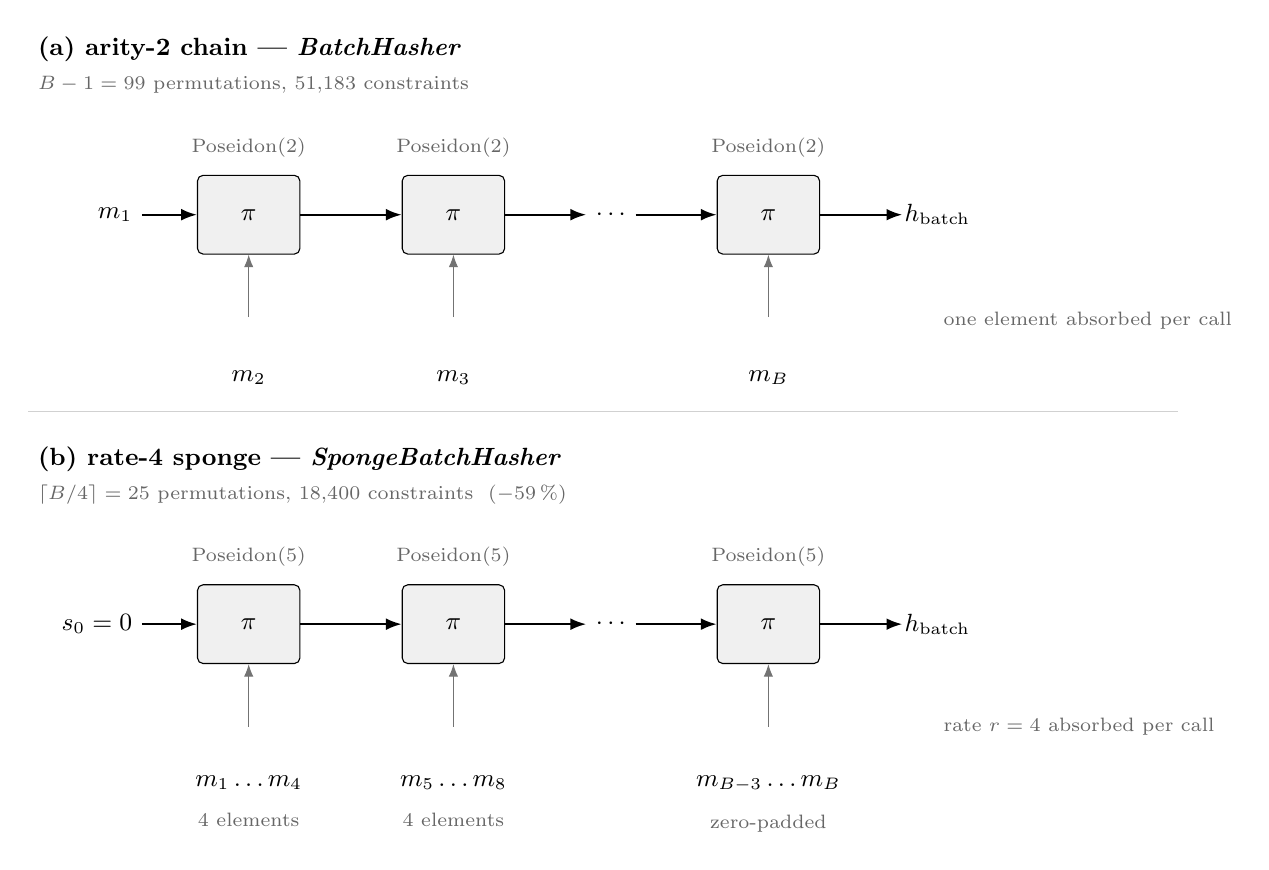
\begin{tikzpicture}[
  font=\small,
  perm/.style={draw, rounded corners=2pt, fill=black!6,
               minimum width=13mm, minimum height=10mm},
  st/.style={-{Latex[length=2mm]}, thick},
  ab/.style={-{Latex[length=1.6mm]}, draw=black!55},
  lbl/.style={font=\scriptsize, text=black!60},
  hd/.style={font=\small\bfseries},
]

% ================= (a) arity-2 chain =================
\node[hd, anchor=west] at (-1.2,2.1) {(a) arity-2 chain \textemdash\ \textit{BatchHasher}};
\node[lbl, anchor=west] at (-1.2,1.65) {$B-1 = 99$ permutations, 51{,}183 constraints};

\node[perm] (a1) at (1.6,0) {$\pi$};
\node[perm] (a2) at (4.2,0) {$\pi$};
\node      (ad) at (6.2,0) {$\cdots$};
\node[perm] (a3) at (8.2,0) {$\pi$};

\node[lbl, above=1mm of a1] {Poseidon(2)};
\node[lbl, above=1mm of a2] {Poseidon(2)};
\node[lbl, above=1mm of a3] {Poseidon(2)};

\node[left=7mm of a1] (am1) {$m_1$};
\draw[st] (am1) -- (a1);
\draw[st] (a1) -- (a2);
\draw[st] (a2) -- (ad);
\draw[st] (ad) -- (a3);
\draw[st] (a3) -- ++(1.7,0) node[right=-1mm] {$h_{\mathrm{batch}}$};

\foreach \n/\m in {a1/m_2, a2/m_3, a3/m_B} {
  \draw[ab] ($(\n)+(0,-1.3)$) -- (\n);
  \node[below=1.35cm of \n, font=\small] {$\m$};
}
\node[lbl, anchor=west] at (10.3,-1.35) {one element absorbed per call};

% ================= (b) rate-4 sponge =================
\draw[black!18] (-1.2,-2.5) -- (13.4,-2.5);

\node[hd, anchor=west] at (-1.2,-3.1) {(b) rate-4 sponge \textemdash\ \textit{SpongeBatchHasher}};
\node[lbl, anchor=west] at (-1.2,-3.55)
  {$\lceil B/4 \rceil = 25$ permutations, 18{,}400 constraints \ ($-59\,\%$)};

\node[perm] (b1) at (1.6,-5.2) {$\pi$};
\node[perm] (b2) at (4.2,-5.2) {$\pi$};
\node      (bd) at (6.2,-5.2) {$\cdots$};
\node[perm] (b3) at (8.2,-5.2) {$\pi$};

\node[lbl, above=1mm of b1] {Poseidon(5)};
\node[lbl, above=1mm of b2] {Poseidon(5)};
\node[lbl, above=1mm of b3] {Poseidon(5)};

\node[left=7mm of b1] (bs0) {$s_0=0$};
\draw[st] (bs0) -- (b1);
\draw[st] (b1) -- (b2);
\draw[st] (b2) -- (bd);
\draw[st] (bd) -- (b3);
\draw[st] (b3) -- ++(1.7,0) node[right=-1mm] {$h_{\mathrm{batch}}$};

\foreach \n/\m/\c in {%
  b1/{m_1\dots m_4}/{4 elements},
  b2/{m_5\dots m_8}/{4 elements},
  b3/{m_{B-3}\dots m_B}/{zero-padded}} {
  \draw[ab] ($(\n)+(0,-1.3)$) -- (\n);
  \node[below=1.3cm of \n, font=\small] (lab\n) {$\m$};
  \node[lbl, below=0.5mm of lab\n] {\c};
}
\node[lbl, anchor=west] at (10.3,-6.5) {rate $r=4$ absorbed per call};

\end{tikzpicture}
\end{document}
